\documentclass[a4paper, 11pt, final, garamond]{book}
\usepackage{cours-preambule}
\usepackage[french]{babel}

\raggedbottom

\makeatletter
\renewcommand{\@chapapp}{Induction -- chapitres}
\renewcommand\thechapter{1 et 2}
\makeatother

\begin{document}
% \setcounter{chapter}{2}

\chapter{Correction du TD}

\section{Aimant en U}
\label{sec:exaimu}
\noindent
\begin{minipage}[t]{.5\linewidth}
  Voir Figure~\ref{fig:exaimucorr}. Les LdC sortent par le Nord, entrent par le
  Sud. Le champ est fort là où les LdC sont serrées, faible là où elles sont
  éloignées. Il est uniforme là où les LdC sont parallèles et régulièrement
  espacées. Dans l'entrefer (\textbf{dans le métal}), le champ va du Sud au
  Nord.
  \bigbreak
  On peut créer des champs uniformes dans un solénoïde, et au milieu d'une
  bobine de \textsc{Helmoltz}, constituée de deux bobines plates de même rayon
  $R$ et espacées de $R$, parcourues par la même intensité dans le même sens.
\end{minipage}
\begin{minipage}[t]{.5\linewidth}
  ~
  \vspace*{-10pt}
  \begin{center}
    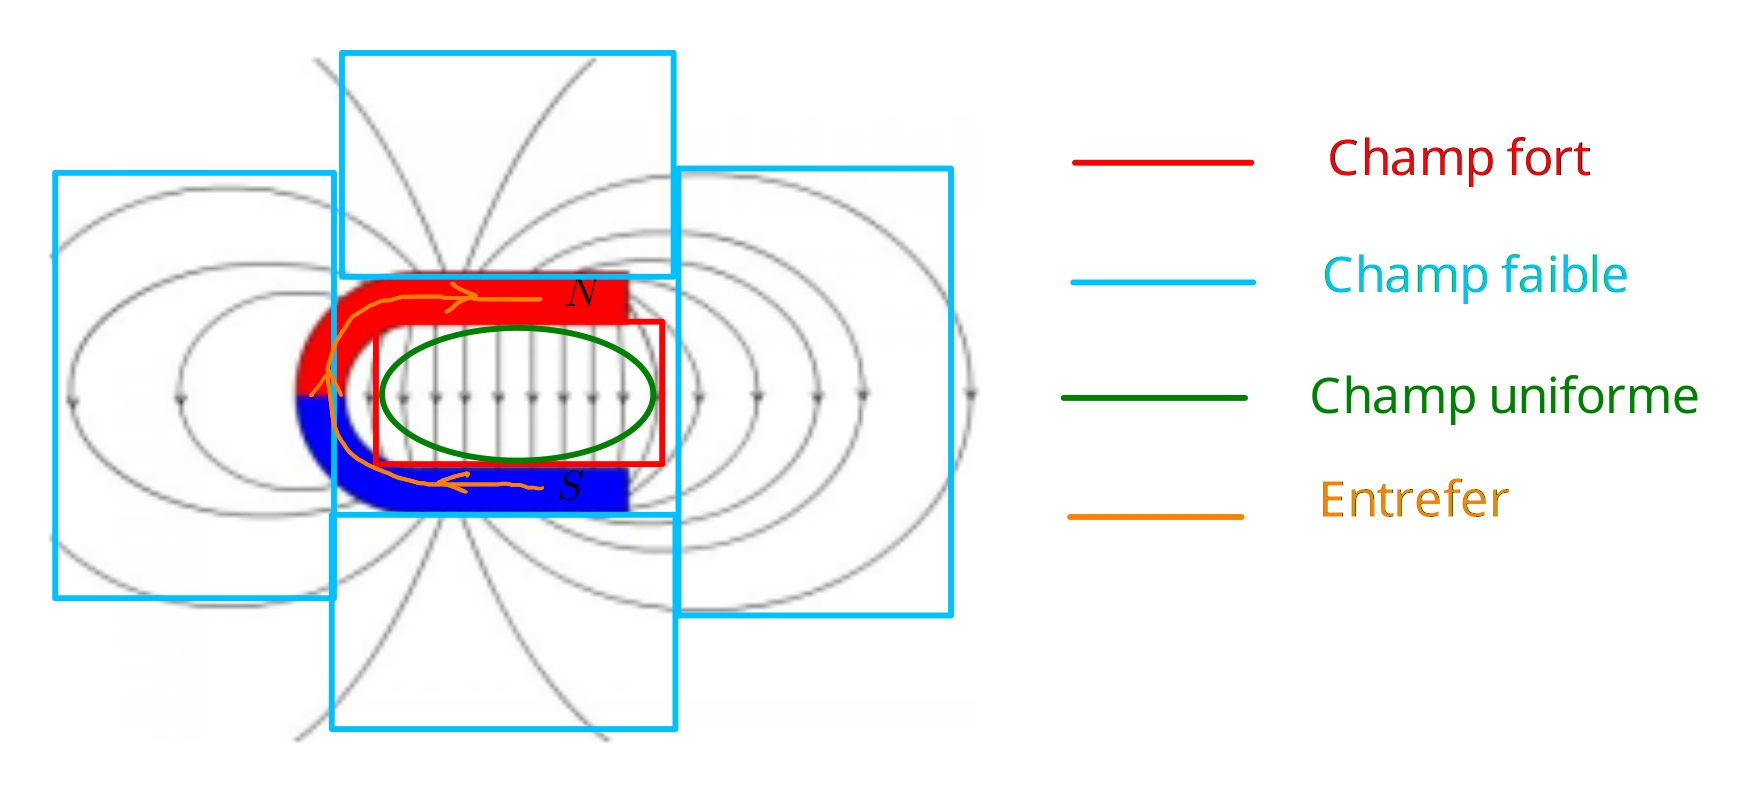
\includegraphics[width=\linewidth]{exaimu_corr}
    \captionof{figure}{Correction aimant en U.}
    \label{fig:exaimucorr}
  \end{center}
\end{minipage}

\section{Cartes de champ}
\label{sec:excchp}
Voir Figure~\ref{fig:excchpcorr}.
\begin{itemize}[label=$\diamond$, leftmargin=10pt]
  \item Le champ est le plus intense là où les LdC sont très rapprochées, et
    faible là où il y a peu de LdC.
  \item Les LdC s'enroulent autour des sources, qui sont donc situées au niveau
    des points noirs de chaque figure. Il y en a six sur la figure de gauche, et
    4 sur la figure de droite. Comme on nous indique que ce sont des spires, on
    a \textbf{3 spires} à gauche et \textbf{2 spires} à droite.
  \item Connaissant l'enroulement des LdC, le sens du courant dans les fils se
    déduit de la règle de la main droite (l'enroulement des doigts donne le sens
    des LdC, le pouce donne le sens du courant). Dans tous les cas, le courant
    est perpendiculaire au plan de la feuille.
    \smallbreak
    Sur la carte de gauche, le courant sort du plan de la feuille $\odot$ pour
    les 3 sources de gauche, et rentrent dans le plan de la feuille $\otimes$
    pour les 3 sources de droite.
    \smallbreak
    Sur la carte de droite, le courant sort du plan de la feuille $\odot$ en haut à
    droite et en bas à gauche, et rentre $\otimes$ en haut à gauche et en bas à
    droite.
\end{itemize}

\begin{figure}[h]
  \centering
  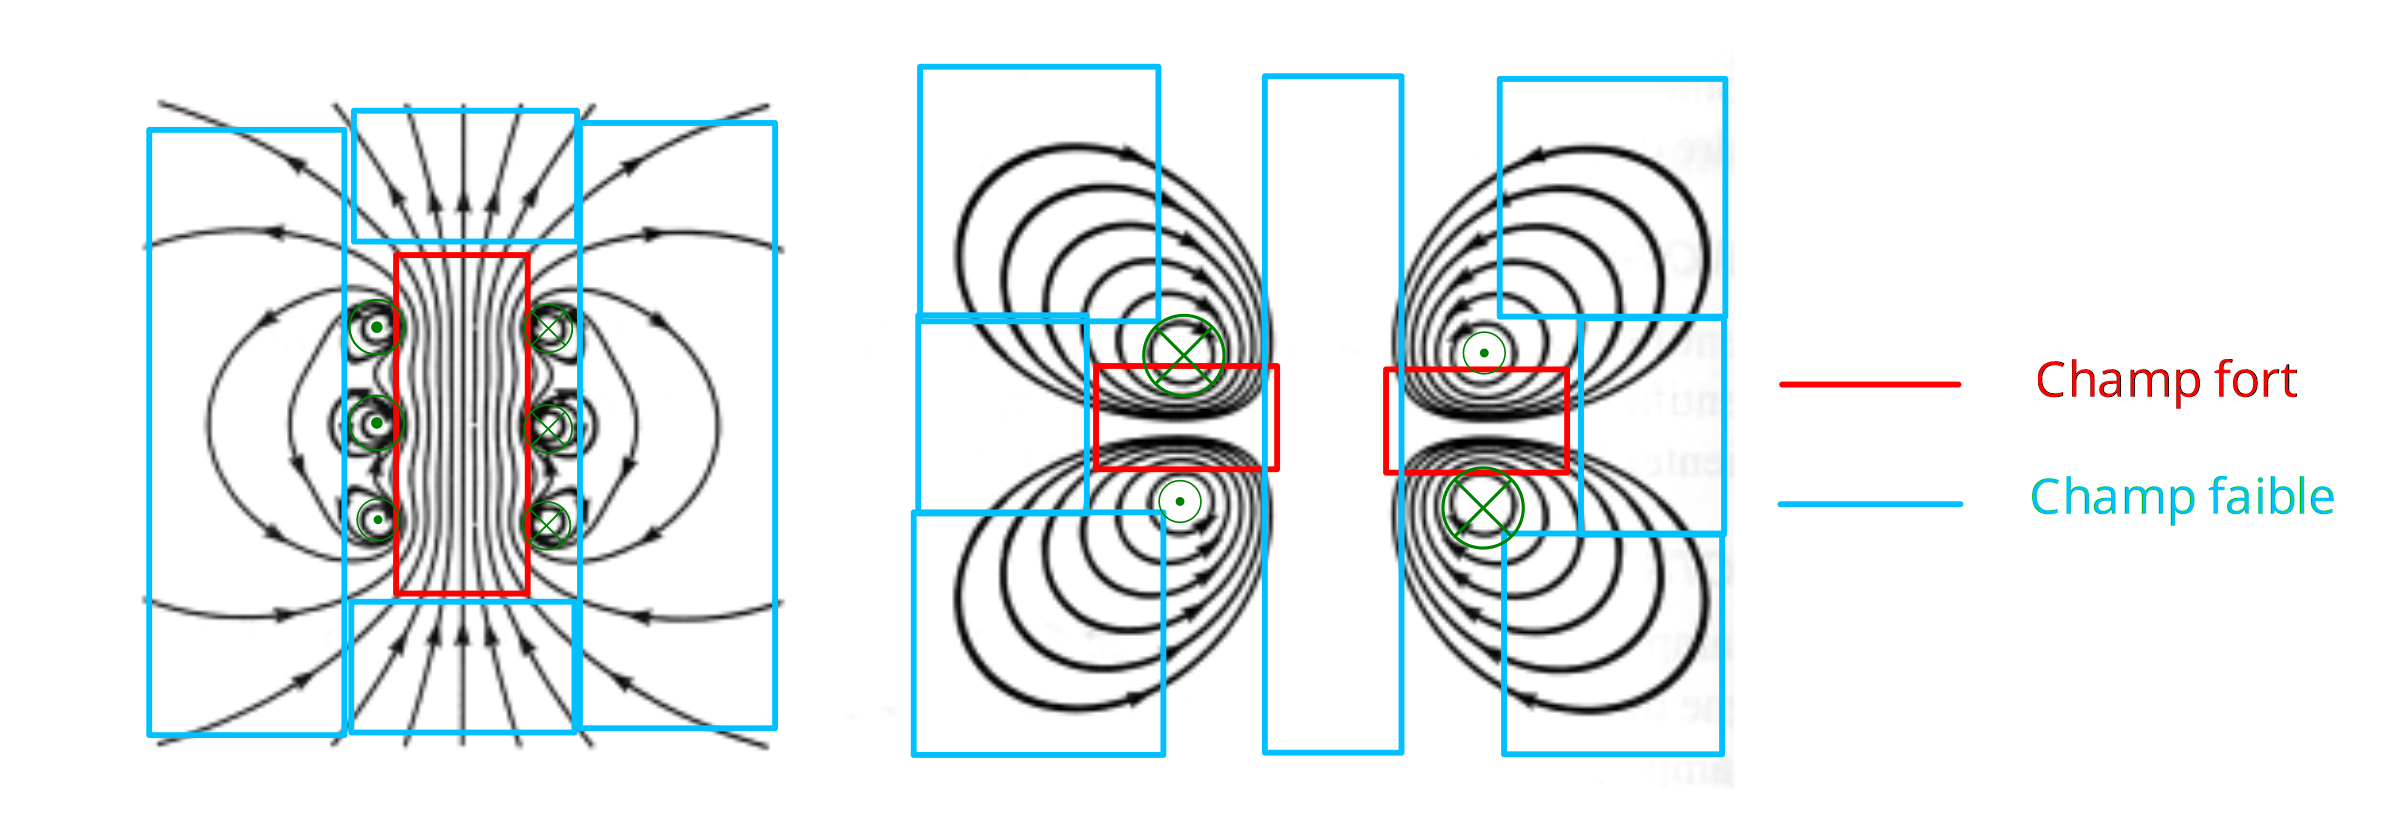
\includegraphics[width=\linewidth]{cchp_corr}
  \caption{Correction cartes de champ.}
  \label{fig:excchpcorr}
\end{figure}

\section{Aimantation d'un matériau}
\label{sec:aimat}
\begin{enumerate}
  \item Le moment magnétique d'une spire plane d'aide $S$ et parcourue par un
    courant $I$ a pour norme $\norm{\vv{\mu}} = SI$. On en déduit qu'un moment
    magnétique s'exprime en \si{A.m^2}. En divisant par un volume en \si{m^3},
    on obtient bien des \si{A.m^{-1}}.
  \item Un aimant est d'autant meilleur que son moment magnétique est élevé et
    son volume faible~: un bon aimant doit donc être fait d'un matériau qui
    possède une \textbf{forte aimantation}.
  \item Pour une aimantation $M = \SI{3e6}{A.m ^{-1}}$, le moment magnétique de
    l'aimant en question vaut
    \[
      \boxed{\mu_{\rm aimant} = M\times\pi R^2 e = \SI{0.2}{A.m^2}}
    \]
  \item Le moment magnétique d'un ensemble de $N$ spires juxtaposées montées en
    série vaut $\mu_{\rm spires} = NI\pi R^2$. Pour avoir le même moment que l'aimant
    précédent, on doit avoir
    \[
      \mu_{\rm aimant} = \mu_{\rm spires}
      \Lra 
      M\pi R^2 e = NI\pi R^2
      \qso
      \boxed{N = \frac{Me}{I} = \num{3e4}}
    \]
    c'est-à-dire \num{30000} spires~! On retiendra qualitativement que le
    magnétisme de la matière est bien plus fort que le magnétisme des courants.
\end{enumerate}

\section{Équilibre d'un aimant}
\label{sec:exeqaim}
\noindent
\begin{minipage}[t]{.6\linewidth}
  \begin{itemize}[label=$\diamond$, leftmargin=10pt]
  \litem{Système~:} \{aimant\} de masse $m$ de moment magnétique $\vv{\mu}$ dans
  un champ $\Bf$.
  \litem{Schéma~:}
  \litem{Modélisation~:}
    \begin{itemize}[label=$\triangleright$, leftmargin=10pt]
      \item Repère~: cartésien, $\uy$ direction de $\Bf$
          soit $\Bf = B\uy$, $\ux$ direction de $\vv{\mu}$ soit $\vv{\mu}
          = \mu \ux$.
      \item Instant initial~: l'aimant est parallèle au sol.
    \end{itemize}
  \litem{BdF~:}
    \[
      \begin{array}{ll}
        \textbf{Poids} & \vv{P} = -mg \uy
        \\
        \textbf{Réaction du support} & \text{passe par O}
      \end{array}
    \]
  \end{itemize}
\end{minipage}
\hfill
\begin{minipage}[t]{.39\linewidth}
  ~
  \vspace*{-10pt}
  \begin{center}
    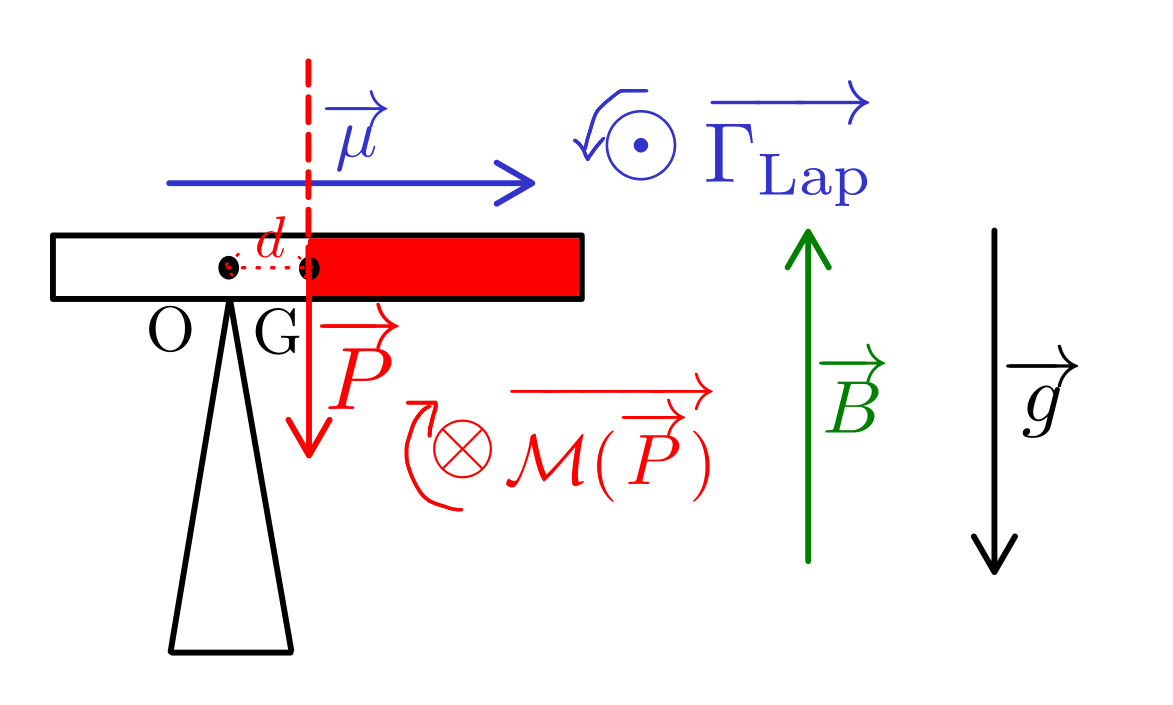
\includegraphics[width=\linewidth]{exeqaim_corr}
    \captionof{figure}{Forces et moments s'appliquant sur l'aimant.}
    \label{fig:exeqaimcorr}
  \end{center}
\end{minipage}
\smallbreak
\begin{itemize}[label=$\diamond$, leftmargin=10pt]
\litem{BdM~:}
  On s'intéresse au moment des forces s'appliquant sur le système. On obtient
  directement le couple magnétique avec la formule démontrée dans le cours
  entre un moment magnétique $\vv{\mu}$ et un champ magnétique $\vv{B}$. Pour
  le poids, on utilise le bras de levier~:
  \begin{itemize}
    \item On prolonge la droite d'action, c'est-à-dire la flèche représentant
      le poids~;
    \item On cherche le projeté orthogonal de l'axe de rotation sur cette
      droite d'action, en prenant une droite perpendiculaire à la droite
      d'action et en trouvant quand elle passe par l'axe~;
    \item La distance obtenue correspond au \textbf{bras de levier}, qu'on
      appelle $d$ ici.
  \end{itemize}
  On a alors
  \[
    \Mc_z(\vv{P}) = \pm d \times mg
  \]
  avec $\pm $ selon que le poids fasse tourner le système dans le sens direct
  (+) ou horaire (-). Ici, le poids a tendance à faire tourner le système dans
  le sens horaire.
  \smallbreak
  Pour le couple magnétique, \textbf{un moment magnétique tend à s'aligner sur
  le champ magnétique}, donc ici tend à faire tourner l'aimant dans le sens
  direct pour s'aligner sur $\vv{B}$.
  \smallbreak
  Pour la réaction du support, elle passe par O donc son moment est nul (pour
  rappel, mathématiquement $\vv{\Mc(\vv{F})} = \vv{\rm OM}\wedge \vv{F}$, donc
  si la force passe par l'axe de rotation on a un moment nul. Équivalent à
  avoir un bras de levier nul). Ainsi,
  \[
    \begin{array}{ll}
      \textbf{Moment du poids} & \Mc(\vv{P}) = -d\times mg
      \\
      \textbf{Moment de la réaction} & \vv{\Mc(\vv{R})} = \vv{0}
      \\
      \textbf{Couple magnétique} &
      \Gamma_{z, \rm Lap} = (\vv{\mu} \wedge \vv{B})\cdot \uz
      \\
      \Lra & \Gamma_{z, \rm Lap} = +\mu B
    \end{array}
  \]
\litem{TMC à l'équilibre~:}
  \begin{align*}
    \dv{\Lc_z}{t} = 0 &= \sum_{i} \Mc_i
    \\\Lra 
    0 &= \Gamma_{z, \rm Lap} + \Mc_{z}(\vv{P})
    \\\Lra 
    0 &= \mu B - dmg
    \\\Lra 
    \Aboxed{d &= \frac{\mu B}{mg}}
  \end{align*}
\end{itemize}

\section{Rails de \textsc{Laplace} inclinés}
\label{sec:railpl}
\begin{enumerate}
  \item Le dispositif est représenté vu de côté et vu de dessus
    Figures~\ref{fig:rlplincl_a} et \ref{fig:rlplincl_b}. On prend les axes
    $x$ et $y$ dans le plan des rails, $z$ perpendiculaire. Outre son poids et
    la force de \textsc{Laplace}, le barreau est également soumis à la réaction
    des rails, perpendiculaire aux rails car les frottements sont négligés.
    \smallbreak
    \noindent
    \begin{minipage}[c]{.45\linewidth}
      ~
      \begin{center}
        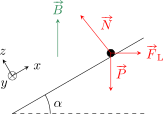
\includegraphics[scale=1]{lplinc_a}
        \label{fig:rlplincl_a}
        \captionof{figure}{Vue de côté.}
      \end{center}
    \end{minipage}
    \hfill
    \begin{minipage}[c]{.45\linewidth}
      ~
      \begin{center}
        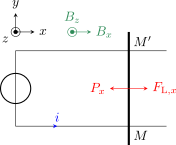
\includegraphics[scale=1]{lplinc_b}
        \label{fig:rlplincl_b}
        \captionof{figure}{Vue de dessus.}
      \end{center}
    \end{minipage}
    \smallbreak
    Pour que la force de \textsc{Laplace} puisse retenir le barreau mobile, il
    faut avoir vectoriellement $\vv{F_L} + \vv{P} + \vv{N} = \vv{0}$. Sur $\uz$
    on va trouver que la réaction compense $\vv{P_z}$ et $\vv{F_{L,z}}$ les
    composantes sur $\uz$ du poids et de la force de \textsc{Laplace}, et sur
    $\ux$ on veut que $\vv{F_{L,x}}$ compense $\vv{P_x}$.
    \smallbreak
    On cherche donc le sens de $i$ qui va donner la force de \textsc{Laplace}
    avec une composante positive sur $\ux$. Avec le sens indiqué sur le schéma,
    la force exercée sur le barreau $\rm MM'$ est
    \[
      \vv{F_L} = i \vv{\rm MM'} \wedge \vv{B}
    \]
    et avec la règle de la main droite version 3 doigts, on trouve bien une
    force de \textsc{Laplace} vers la droite. Le courant doit donc effectivement
    être \textbf{dirigé de M à M'} pour retenir le barreau.
  \item Le poids du barreau mobile à pour norme $mg$, et la force de
    \textsc{Laplace} $i \ell B$. En projection sur $\ux$, on trouve
    \[
      i \ell B \cos{\alpha} = mg \sin{\alpha}
      \qso
      \boxed{i = \frac{mg \tan{\alpha}}{\ell B} = \SI{2.5}{A}}
    \]
  \item Si les frottements et l'induction sont négligés, alors le bilan des
    forces est exactement le même que précédemment~: leur résultante est nulle.
    On garde donc le PFD à l'équilibre
    \[
      \dv{\vv{p}}{t} = \vv{0}
    \]
    mais cette fois $\vv{v_0} \neq \vv{0}$. On garde donc cette vitesse
    constante, et \textbf{le barreau aura un mouvement rectiligne uniforme vers
    le haut à la vitesse $v_0$}.
  \item D'après la loi de \textsc{Lenz}, l'induction modère, par ses
    conséquences, les causes qui lui ont donné naissance.
    \smallbreak
    Ici, c'est le mouvement du barreau parcouru par $i$ et dans un champ
    $\vv{B}$ qui causera l'induction, par modification de la surface du circuit
    (la surface qu'entoure l'intensité augmente). On aura donc \textit{in fine}
    une force de \textsc{Laplace} induite qui s'opposera au mouvement du
    barreau, donc \textbf{le barreau va freiner jusqu'à son arrêt}, puisqu'alors
    la surface ne variera plus.
\end{enumerate}

\section{Mesure du champ magnétique terrestre}
\label{sec:meschpterre}
\begin{enumerate}
  \item Le champ magnétique terrestre est de l'ordre de \SI{5e-5}{T}. Or, le
    teslamètre ne permet pas de mesurer des champs inférieurs à \SI{1e-4}{T}.
  \item À partir de l'expression données, on trouve $B = \SI{1e-5}{T}$.
  \item Placer le dispositif d'\textsc{Œrsted} selon une direction Nord-Sud, de
    telle sorte que l'aiguille soit parallèle au fil lorsqu'il n'est parcouru
    par aucun courant. Relier le fil d'\textsc{Œrsted} à l'interrupteur et à
    l'alimentation stabilisée, de telle sorte qu'il puisse être alimenté par un
    courant constant. Placer le rapporteur de sorte à pouvoir mesurer la
    déviation de l'aiguille lorsque l'interrupteur est fermé, et inclure
    l'ampèremètre dans le circuit pour pouvoir mesurer l'intensité du courant.
    \begin{figure}[h]
      \centering
      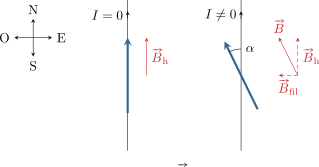
\includegraphics[scale=1]{magTorst}
      \caption{Schéma de principe de l'expérience. Le sens de
      $\protect\vv{B_{\rm fil}}$ est obtenu à partir de la règle de la main
    droite, en raisonnant en vue de dessus avec l'aiguille aimantée placée
  en-dessous du fil.}
      \label{fig:orstedcorr}
    \end{figure}
    L'aiguille étant à une distance fixe du fil, on suppose que le champ créé
    est homogène. Le moment magnétique de l'aiguille va donc s'orienter sur ce
    champ, entrant en compétition avec le champ magnétique terrestre.
  \item L'aiguille s'aligne sur le champ total, superposition du champ du fil et
    du champ terrestre. Le dispositif est monté de telle sorte que les deux
    champs soient orthogonaux, si bien qu'on peut relier directement
    \[
      \tan{\alpha} = \frac{B_{\rm fil}}{B_{\rm h}}
    \]
    En mesurant $\alpha$ pour différentes valeurs de $I$ à partir desquelles on
    en déduit $B_{\rm fil}$, on peut alors obtenir $B_{\rm h}$ par une
    régression linéaire. On peut par exemple représenter $B_{\rm fil}$ en
    fonction de $\tan{\alpha}$.
  \item Compte-tenu de l'expression donnée et pour une aiguille située
    \SI{2}{cm} sous le fil, il faudrait avoir $I = \SI{5}{A}$ pour que $B_{\rm
    fil} = B_{\rm h}$.
\end{enumerate}

\end{document}
